%%%%%%%%%%%%%%%%%%%%%%%%%%%%%%%%%%%%%%%%%%%%%%%%%%%%%%%%
%%
\clearpage
\newpage
\section{The cal\_DRIFT recipes}
\label{ch:the_recipes:cal_DRIFT_RAW_spirou}
%%
%%%%%%%%%%%%%%%%%%%%%%%%%%%%%%%%%%%%%%%%%%%%%%%%%%%%%%%%

There are currently three different drift recipes: \calDRIFTRAW, \calDRIFTE and \calDRIFTPEAK. The \calDRIFTE and \calDRIFTPEAK\, recipes are the primary drift code recipes and \calDRIFTRAW is an older version where spectra are re-extracted.

% -------------------------------------------------------
\subsection{The inputs}
% -------------------------------------------------------

\subsubsection{cal\_DRIFT\_E2DS\_spirou and cal\_DRIFTPEAK\_E2DS\_spirou}

The input of \calDRIFTE and \calDRIFTPEAK are as follows:
\begin{cmdbox}
cal_DRIFT_E2DS_spirou.py night_repository referenece_file
cal_DRIFTPEAK_E2DS_spirou.py night_repository referenece_file
\end{cmdbox}
\noindent for example
\begin{cmdbox}[title={example}]
cal_DRIFT_E2DS_spirou.py 20170710 fp_fp02a203_e2ds_AB.fits
cal_DRIFTPEAK_E2DS_Spirou.py 20170710 fp_fp02a203_e2ds_AB.fits
\end{cmdbox}
\noindent or
\begin{pythonbox}
import cal_DRIFT_E2DS_spirou
import cal_DRIFTPEAK_E2DS_Spirou
night_repository = '20170710'
reffilename = 'fp_fp02a203_e2ds_AB.fits'
cal_DRIFT_E2DS_spirou.main(night_repository, reffile=reffilename)
cal_DRIFTPEAK_E2DS_Spirou.main(night_repository, reffile=reffilename)
\end{pythonbox}

\noindent where `night\_repository' defines \argnightname and `refilename' define the file to use as the reference spectrum. The reference file must be a valid python string and must have the folowing prefixes:
\begin{itemize}
	\item fp\_fp
\end{itemize}
\noindent and must contain the fiber type (i.e. `AB' or `A' or `C').

% - - - - - - - - - - - - - - - - - - - - - - - - - - - -

\subsubsection{cal\_DRIFT\_RAW\_spirou}

The input of \calDRIFTRAW is as follows:
\begin{cmdbox}
cal_DRIFT_RAW_spirou.py night_repository files
\end{cmdbox}
\noindent for example
\begin{cmdbox}[title={example}]
cal_DRIFT_RAW_spirou.py 20170710 fp_fp02a203.fits
\end{cmdbox}
\noindent or
\begin{pythonbox}
import cal_DRIFT_RAW_spirou
night_repository = '20170710'
filenames = ['fp_fp02a203.fits']
cal_DRIFT_RAW_spirou.main(night_repository, files=filenames)
\end{pythonbox}

\noindent where `night\_repository' defines \argnightname and `filenames' define the list of files in \argfilenames. All files in filenames must be valid python strings separated by a space (command line) or in a line (python) and must have the folowing prefixes:
\begin{itemize}
	\item fp\_fp
\end{itemize}

\begin{note}
\calDRIFTRAW can also take an addition argument. By default it will extract fiber `AB', but this can be changed if using python by specifying the `fiber' keyword, for example:
\begin{pythonbox}
import cal_DRIFT_RAW_spirou
night_repository = '20170710'
filenames = ['fp_fp02a203.fits']
cal_DRIFT_RAW_spirou.main(night_repository, files=filenames, fiber='A')
\end{pythonbox}
\end{note}

% -------------------------------------------------------
\subsection{The outputs}
% -------------------------------------------------------

\subsubsection{cal\_DRIFT\_E2DS\_spirou}

The outputs of \calDRIFTE is as follows:

\begin{itemize}

\item \definevariable{text:driftfits_e2ds}{driftfits\_e2ds} in form:
\begin{tcustomdir}
\{\reduceddir\}/\{date prefix\}\_\{file\}\_drift\_\{fiber\}.fits
\end{tcustomdir}

\item \definevariable{text:drifttblfilename_e2ds}{drifttblfilename\_e2ds} in form:
\begin{tcustomdir}
\{\reduceddir\}/\{date prefix\}\_\{file\}\_drift\_\{fiber\}.tbl
\end{tcustomdir}

\end{itemize}


\noindent where `date prefix' is constructed from \argnightname and the file name is the `reference filename'.


\noindent for example for \reduceddir\lstinline[style=pythoninline]|='/drs/data/reduced/20170710'|, \lstinline[style=pythoninline]|reffile = 'fp_fp02a203_e2ds_AB.fits'| and \lstinline[style=pythoninline]|fiber='AB'| the output files would be:
\begin{tcustomdir}
\begin{itemize}
\item \path{/drs/data/reduced/20170710/fp_fp02a203_e2ds_AB_drift_AB.fits}
\item \path{/drs/data/reduced/20170710/fp_fp02a203_e2ds_AB_drift_AB.tbl}
\end{itemize}
\end{tcustomdir}


% - - - - - - - - - - - - - - - - - - - - - - - - - - - -
\subsubsection{cal\_DRIFTPEAK\_E2DS\_spirou}

The outputs of \calDRIFTPEAK is as follows:

\begin{itemize}

\item \definevariable{text:driftfits_peak_e2ds}{driftfits\_peak\_e2ds} in form:
\begin{tcustomdir}
\{\reduceddir\}/\{date prefix\}\_\{file\}\_driftnew\_\{fiber\}.fits
\end{tcustomdir}

\item \definevariable{text:drifttblfilename_peak_e2ds}{drifttblfilename\_peak\_e2ds} in form:
\begin{tcustomdir}
\{\reduceddir\}/\{date prefix\}\_\{file\}\_driftnew\_\{fiber\}.tbl
\end{tcustomdir}

\end{itemize}


\noindent where `date prefix' is constructed from \argnightname and the file name is the `reference filename'.


\noindent for example for \reduceddir\lstinline[style=pythoninline]|='/drs/data/reduced/20170710'|, \lstinline[style=pythoninline]|reffile = 'fp_fp02a203_e2ds_AB.fits'| and \lstinline[style=pythoninline]|fiber='AB'| the output files would be:
\begin{tcustomdir}
\begin{itemize}
\item \path{/drs/data/reduced/20170710/fp_fp02a203_e2ds_AB_driftnew_AB.fits}
\item \path{/drs/data/reduced/20170710/fp_fp02a203_e2ds_AB_driftnew_AB.tbl}
\end{itemize}
\end{tcustomdir}

% - - - - - - - - - - - - - - - - - - - - - - - - - - - -
\subsubsection{cal\_DRIFT\_RAW\_spirou}

The outputs of \calDRIFTRAW are as follows:

\begin{itemize}

\item \definevariable{text:driftfits_raw}{driftfits\_raw} in form:
\begin{tcustomdir}
\{\reduceddir\}/\{date prefix\}\_\{file\}\_drift\_\{fiber\}.fits
\end{tcustomdir}

\end{itemize}


\noindent where `date prefix' is constructed from \argnightname and the file name is the first file in \argfilenames.


\noindent for example for \reduceddir\lstinline[style=pythoninline]|='/drs/data/reduced/20170710'|, \argfilenames\lstinline[style=pythoninline]|=['fp_fp02a203.fits']| and \lstinline[style=pythoninline]|fiber='AB'| the output files would be:
\begin{tcustomdir}
\begin{itemize}
\item \path{/drs/data/reduced/20170710/fp_fp02a203_e2ds_AB_drift_AB.fits}
\end{itemize}
\end{tcustomdir}


% -------------------------------------------------------
\subsection{Summary of procedure}
% -------------------------------------------------------

\subsubsection{cal\_DRIFT\_E2DS\_spirou}

\begin{enumerate}
	\item first file is reference image (must be an E2DS file) extracted using one of the cal\_extract\_RAW recipes
	\item loops around all other `*\_e2ds\_\{fiber\}.fits' files in directory
	\item calculates photon noise uncertainty and estimated RV uncertainty on spectrum
	\begin{itemize}
		\item uses wave file
	\end{itemize}
	\item calculates RV drift and mean RV drift between reference (mean of files) and other `fp\_fp' files
	\item saves drift values to file
\end{enumerate}

% - - - - - - - - - - - - - - - - - - - - - - - - - - - -
\subsubsection{cal\_DRIFTPEAK\_E2DS\_spirou}

\begin{enumerate}
	\item first file is reference image
	\item resizes the image
	\item background correction
	\item Identifies FP peaks in reference file
	\item Creates a reference ascii file that contains the positions of the FP peaks
	\item Removes lines with suspicious widths
	\item loops around all other `*\_e2ds\_\{fiber\}.fits' files
	\item Gets the centroid of all peaks using Gaussian fitting
	\item Performs a Pearson R test to look for issues with extraction and/or illumination
	\item Performs sigma clipping on measured drift
	\item Saves drifts to file
\end{enumerate}

% - - - - - - - - - - - - - - - - - - - - - - - - - - - -
\subsubsection{cal\_DRIFT\_RAW\_spirou}
\begin{enumerate}
	\item first file is reference image
	\item resizes the image
	\item extracts with weight (no tilt)
	\item loops around all other `fp\_fp' files in directory
	\item calculates photon noise uncertainty and estimated RV uncertainty on spectrum
	\begin{itemize}
		\item uses wave file
	\end{itemize}
	\item calculates RV drift and mean RV drift between reference (mean of files) and other `fp\_fp' files
	\item saves drift values to file
\end{enumerate}


% -------------------------------------------------------
\newpage
\subsection{Example working run}
% -------------------------------------------------------

\subsubsection{cal\_DRIFT\_E2DS\_spirou}

An example run where everything worked is below:
\begin{cmdbox}[title={example}]
cal_DRIFT_E2DS_spirou.py 20170710 fp_fp02a203_e2ds_AB.fits
\end{cmdbox}
\begin{cmdboxprintspecial}[fontupper=\tiny, fontlower=\tiny]
@g

@g
\end{cmdboxprintspecial}



% - - - - - - - - - - - - - - - - - - - - - - - - - - - -
\subsubsection{cal\_DRIFTPEAK\_E2DS\_spirou}

An example run where everything worked is below:
\begin{cmdbox}[title={example}]
cal_DRIFTPEAK_E2DS_Spirou.py 20170710 fp_fp02a203_e2ds_AB.fits
\end{cmdbox}
\begin{cmdboxprintspecial}[fontupper=\tiny, fontlower=\tiny]
@g

@g
\end{cmdboxprintspecial}


% - - - - - - - - - - - - - - - - - - - - - - - - - - - -
\subsubsection{cal\_DRIFT\_RAW\_spirou}

\begin{cmdbox}[title={example}]
cal_DRIFT_RAW_spirou.py 20170710 fp_fp02a203.fits
\end{cmdbox}
\begin{cmdboxprintspecial}[fontupper=\tiny, fontlower=\tiny]
@gHH:MM:SS.S -   || *****************************************@g
@gHH:MM:SS.S -   || * SPIROU \@(#) Geneva Observatory (VERSION)@g
@gHH:MM:SS.S -   || *****************************************@g
@gHH:MM:SS.S -   ||(dir_data_raw)      DRS_DATA_RAW=/drs/data/raw@g
@gHH:MM:SS.S -   ||(dir_data_reduc)    DRS_DATA_REDUC=/drs/data/reduced@g
@gHH:MM:SS.S -   ||(dir_calib_db)      DRS_CALIB_DB=/drs/data/calibDB@g
@gHH:MM:SS.S -   ||(dir_data_msg)      DRS_DATA_MSG=/drs/data/msg@g
@gHH:MM:SS.S -   ||(print_level)       PRINT_LEVEL=all         %(error/warning/info/all)@g
@gHH:MM:SS.S -   ||(log_level)         LOG_LEVEL=all         %(error/warning/info/all)@g
@gHH:MM:SS.S -   ||(plot_graph)        DRS_PLOT=1            %(def/undef/trigger)@g
@gHH:MM:SS.S -   ||(used_date)         DRS_USED_DATE=undefined@g
@gHH:MM:SS.S -   ||(working_dir)       DRS_DATA_WORKING=/drs/data/tmp@g
@gHH:MM:SS.S -   ||                    DRS_INTERACTIVE is not set, running on-line mode@g
@gHH:MM:SS.S -   ||                    DRS_DEBUG is set, debug mode level:1@g
@gHH:MM:SS.S -   |cal_DRIFT_RAW_spirou:2a203|Now running : cal_DRIFT_RAW_spirou on file(s): fp_fp02a203.fits@g
@gHH:MM:SS.S -   |cal_DRIFT_RAW_spirou:2a203|On directory /drs/data/raw/20170710@g
@gHH:MM:SS.S -   |cal_DRIFT_RAW_spirou:2a203|ICDP_NAME loaded from: /scratch/Projects/spirou_py3/spirou_py3/INTROOT/config/constants_SPIROU.py@g
@gHH:MM:SS.S - * |cal_DRIFT_RAW_spirou:2a203|Correct type of image for Drift (f or p or _ or f or p)@g
@gHH:MM:SS.S -   |cal_DRIFT_RAW_spirou:2a203|Calibration file: 20170710_flat_flat02f10_badpixel.fits already exists - not copied@g
@gHH:MM:SS.S -   |cal_DRIFT_RAW_spirou:2a203|Calibration file: 20170710_flat_dark02f10_blaze_AB.fits already exists - not copied@g
...
@gHH:MM:SS.S -   |cal_DRIFT_RAW_spirou:2a203|Calibration file: 2017-10-11_21-32-17_hcone_hcone02c406_wave_C.fits already exists - not copied@g
@gHH:MM:SS.S - * |cal_DRIFT_RAW_spirou:2a203|Now processing Image TYPE UNKNOWN with cal_DRIFT_RAW_spirou recipe@g
@gHH:MM:SS.S -   |cal_DRIFT_RAW_spirou:2a203|Reading Image /drs/data/raw/20170710/fp_fp02a203.fits@g
@gHH:MM:SS.S -   |cal_DRIFT_RAW_spirou:2a203|Image 2048 x 2048 loaded@g
@gHH:MM:SS.S -   |cal_DRIFT_RAW_spirou:2a203|Doing Dark Correction using /drs/data/calibDB/20170710_dark_dark02d406.fits@g
@gHH:MM:SS.S -   |cal_DRIFT_RAW_spirou:2a203|Image format changed to 2035x1930@g
@gHH:MM:SS.S - * |cal_DRIFT_RAW_spirou:2a203|Nb dead pixels = 568485 / 14.47 %@g
@gHH:MM:SS.S -   |cal_DRIFT_RAW_spirou:2a203|Reading localization parameters of Fiber AB@g
@gHH:MM:SS.S -   |cal_DRIFT_RAW_spirou:2a203AB|Reading order profile of Fiber AB@g
@gHH:MM:SS.S -   |cal_DRIFT_RAW_spirou:2a203|Extraction Reference file /drs/data/raw/20170710/fp_fp02a203.fits@g
@gHH:MM:SS.S -   |cal_DRIFT_RAW_spirou:2a203|On fiber AB order 0: S/N= 513.5@g
@gHH:MM:SS.S -   |cal_DRIFT_RAW_spirou:2a203|On fiber AB order 1: S/N= 561.6@g
...
@gHH:MM:SS.S -   |cal_DRIFT_RAW_spirou:2a203|On fiber AB order 34: S/N= 283.3@g
@gHH:MM:SS.S -   |cal_DRIFT_RAW_spirou:2a203|On fiber AB order 35: S/N= 149.9@g
@gHH:MM:SS.S - * |cal_DRIFT_RAW_spirou:2a203|On fiber AB estimated RV uncertainty on spectrum is 0.028 m/s@g
@gHH:MM:SS.S - * |cal_DRIFT_RAW_spirou:2a203|Number of fp_fp files found on directory = 2@g
@gHH:MM:SS.S -   |cal_DRIFT_RAW_spirou:2a203|Reading file fp_fp03a203.fits@g
@gHH:MM:SS.S -   |cal_DRIFT_RAW_spirou:2a203|Time from ref=0.09 h  - Drift mean=2.53 m/s - Flux ratio=0.99 = Nb Comsic=1218@g
@gHH:MM:SS.S -   |cal_DRIFT_RAW_spirou:2a203|Reading file fp_fp04a203.fits@g
@gHH:MM:SS.S -   |cal_DRIFT_RAW_spirou:2a203|Time from ref=0.18 h  - Drift mean=-10.13 m/s - Flux ratio=0.98 = Nb Comsic=1246@g
@gHH:MM:SS.S -   |cal_DRIFT_RAW_spirou:2a203|Total drift Peak-to-Peak=12.596 m/s RMS=6.298 m/s in 0.18 hour@g
@gHH:MM:SS.S -   |cal_DRIFT_RAW_spirou:2a203|Saving drift values of Fiber AB in fp_fp02a203_drift_AB.fits@g
@yHH:MM:SS.S - \@ |python warning Line 980  warning reads: Card is too long, comment will be truncated.|@y
@gHH:MM:SS.S - * |cal_DRIFT_RAW_spirou:2a203|Recipe cal_DRIFT_RAW_spirou has been successfully completed@g
\end{cmdboxprintspecial}

% % -------------------------------------------------------
% \newpage
% \subsection{Interactive mode}
% % -------------------------------------------------------

% \noindent In interactive mode three figures will also appear (see Figure \ref{figure:}).

% \begin{figure}

% \begin{center}
% \begin{minipage}{.495\textwidth}
% \begin{center}
% \includegraphics[width=\textwidth]{Figures/cal_DARK_spirou_1.pdf}
% a
% \end{center}
% \end{minipage}%
% \begin{minipage}{.495\textwidth}
% \begin{center}
% \includegraphics[width=\textwidth]{Figures/cal_DARK_spirou_2.pdf}
% b
% \end{center}
% \end{minipage}%
% \end{center}

% \begin{center}
% \begin{minipage}{.495\textwidth}
% \begin{center}
% \includegraphics[width=\textwidth]{Figures/cal_DARK_spirou_3.pdf}
% c
% \end{center}
% \end{minipage}%
% \end{center}

% \caption{\textbf{(a)} The image with overplot red and blue regions (red/blue rectangles). \textbf{(b)} The bad pixel mask, bad pixels have a value=1 (in black) and good pixels have a value=0 (in white). \textbf{(c)} Histograms of the image regions, the full image (in green), the blue section (in blue) and the red section (in red). \label{figure:cal_DARK_spirou}}
% \end{figure}